
%
%    PhD Thesis
% ~~~~~~~~~~~~~~~~~
%  Master Document
%

\documentclass[twoside,openright,12pt]{book}

%  Packages
%***********

% Main
\usepackage[utf8]{inputenc}
\usepackage[UKenglish]{babel}
\usepackage[T1]{fontenc}

% Bibliography
%~ \usepackage[
    %~ backend=biber,
    %~ style=numeric,
    %~ natbib=true,
    %~ url=false,
    %~ doi=true,
    %~ eprint=false
%~ ]{biblatex}
\usepackage[
    square,
    numbers,
    sort&compress
]{natbib}
\bibliographystyle{PhD}
\usepackage{doi}

% Layout
\usepackage{titlesec}
\usepackage{pdfpages}
\usepackage{emptypage}
\usepackage[a4paper]{geometry}
\usepackage{setspace}
\usepackage[garamondx,expert]{mathdesign}
%\usepackage[scaled]{berasans}
%\usepackage[scaled]{beramono}
\usepackage[scaled]{raleway}
\usepackage{textcomp}
\usepackage{tgtermes}
\usepackage{hanging}                      % Used for indented paragraphs
\usepackage{appendix}                     % Added functionality for appendices
\usepackage{fancyhdr}
\usepackage{tocloft}                      % For modifying the Table of Contents
\usepackage{hyperref}                     % Managing links
\usepackage{url}                          % Managing links

% Text

% Math
\usepackage{nicefrac}
%\usepackage{xfrac}

% Colours
\usepackage{color}
\definecolor{chapter}{gray}{0.6}
\definecolor{appendix}{gray}{0.5}
\definecolor{m-blue}  {rgb}{0.000,0.447,0.741}
\definecolor{m-red}   {rgb}{0.850,0.325,0.098}
\definecolor{m-yellow}{rgb}{0.929,0.694,0.125}
\definecolor{m-purple}{rgb}{0.494,0.184,0.556}
\definecolor{m-green} {rgb}{0.466,0.674,0.188}
\definecolor{m-cyan}  {rgb}{0.301,0.745,0.933}
\definecolor{m-brown} {rgb}{0.635,0.078,0.184}

% Disabled
%~ \usepackage{latexsym}
%~ \usepackage{amsmath}
%~ \usepackage{amssymb}
%~ \usepackage{cite}
%~ \usepackage{graphicx}
%~ \usepackage{float}
%~ \usepackage{listings}
%~ \usepackage{simplewick}
%~ \usepackage{datetime}

% Package Settings
%==================

% Links
\hypersetup{colorlinks=true, citecolor=m-blue, urlcolor=m-blue, linkcolor=m-blue}

% Layout
\geometry{twoside,margin=2.5cm}
\renewcommand{\rmdefault}{ptm}
\renewcommand{\sfdefault}{phv}
\renewcommand{\ttdefault}{pcr}
\AtBeginDocument{\parskip=0pt plus 2.5pt\relax\setstretch{1.1}}

% Bibliography
\citeindextrue
%~ \addbibresource{Bibliography.bib}
%~ \AtEveryBibitem{
    %~ %\clearfield{day}
    %~ %\clearfield{month}
    %~ %\clearfield{title}
    %~ %\clearfield{series}
    %~ %\clearfield{note}
    %~ %\clearlist{location}
    %~ %\clearlist{institution}
    %~ %\clearlist{language}
    %~ %\clearname{editor}
%~ }

% Fix section numbering bug in titlesec
\usepackage{etoolbox}
\makeatletter
\patchcmd{\ttlh@hang}{\parindent\z@}{\parindent\z@\leavevmode}{}{}
\patchcmd{\ttlh@hang}{\noindent}{}{}{}
\makeatother

% TOC
\renewcommand\cftpartfont{\sffamily\large}
\renewcommand\cftpartpagefont{\mdseries}
\renewcommand\cftchapfont{\mdseries}
\renewcommand\cftchappagefont{\mdseries}
\renewcommand\cfttoctitlefont{\huge\sffamily}
%\renewcommand{\cftchapleader}{\cftdotfill{\cftdotsep}}

% Custom Commands
%*****************

% Text
\newcommand{\eq}[1]{Eq. \ref{#1}}
\newcommand{\fig}[1]{Fig. \ref{#1}}
\newcommand{\tbl}[1]{Table \ref{#1}}
\newcommand{\ts}[1]{\textsuperscript{#1}}

% Math Commands
\newcommand{\unit}[1]{\,\mathrm{#1}}
\newcommand{\funit}[2]{\,\nicefrac{\mathrm{#1}}{\mathrm{#2}}}
\newcommand{\mexp}[1]{\mathrm{e}^{#1}}
\newcommand{\nexp}[1]{\times 10^{#1}}

% ==================================================================================================================== %

% Page Layout
%*************

% Plain Page Numbering
\fancypagestyle{plain}{
    \fancyhf{}
    \fancyfoot[LE,RO]{\thepage}
}

% Header style for numbered chapters
\newcommand{\defaulthead}{
    \fancyhead[LE]{\nouppercase{\itshape\leftmark}}
    \fancyhead[RO]{\nouppercase{\itshape\rightmark}}
}

% Custom heading for unnumbered chapters
\newcommand{\simplehead}[1]{
    \fancyhead[LE]{\nouppercase{\itshape #1}}
    \fancyhead[RO]{\nouppercase{\itshape #1}}
}

\pagestyle{fancy}

% Page Header
\renewcommand{\chaptermark}[1]{\markboth{\chaptername\ \thechapter\ --\ #1}{}}
\renewcommand{\sectionmark}[1]{\markright{\thesection\ #1}{}}
\renewcommand{\headrulewidth}{0pt}
\renewcommand{\footrulewidth}{0pt}

\fancyhf{}
\defaulthead
\headheight 15pt
\fancyfoot[LE,RO]{\thepage}

% Parts
\titleformat{\part}[block]{}{}{}{\centering\fontsize{40}{50}\sffamily}

% Numbered Chapters
\titlespacing*{\chapter}{0mm}{10mm}{20mm}
\titleformat{\chapter}[hang]%
    {\fontsize{60}{70}\sffamily}%
    {\textcolor{chapter}\thechapter}%
    {8mm}%
    {\huge\sffamily}

% Sections
\titleformat{\section}{\large\sffamily}{\thesection}{2mm}{\large}
\titleformat{\subsection}{\normalsize\sffamily}{\thesubsection}{2mm}{}

% ==================================================================================================================== %

% Main Document
%***************

\begin{document}

% Front Matters

\frontmatter
    \begin{titlepage}
    \begin{center}
        \vspace*{10mm}
        \huge{}
        Preliminary Title:\\
        Plasma Wakefield Acceleration\\
        \vspace{20mm}
        \large
        \textbf{Veronica K. Berglyd Olsen}\\
        Department of Physics\\
        University of Oslo\\
        Norway\\
        \vfill
        \includegraphics[width=0.35\textwidth]{images/UiOLogo.pdf}\\
        \vspace{20mm}
        Dissertation Presented for the Degree of\\
        Philosophiae Doctor (PhD) in Physics\\
        \vspace{10mm}
        \large{July 2017}
    \end{center}
\end{titlepage}

    \chapter*{Abstract}
\label{Abstract}

Plasma wakefield accelerators promise to deliver orders of magnitude higher accelerating gradients than conventional accelerator technology.
Whether the technology is used for even higher energy accelerators than exist today, or more compact accelerators, the promise of high gradients has sparked a number of plasma wakefield experiments over the last few decades.

The Advanced Wakefield Experiment (AWAKE) is the first to exploit the self-modulation instability in long particle bunches in plasma in combination with a proton bunch from an existing high energy synchrotron.
The experiment is located at CERN and connected to the Super Proton Synchrotron (SPS).
The first run of AWAKE saw electrons accelerated from 19 mega-electronvolts (MeV) to 2 giga-electronvolts (GeV) in just 10 metres of ionised Rubidium vapour, achieving a gradient of nearly 200 MV/m.

A challenge facing plasma wakefield accelerator designs is the final quality of the accelerated bunch in terms of its spread in energy and its emittance.
In order to minimise both these parameters while retaining a high accelerating gradient -- goals that are to an extent in conflict -- the electron bunch needs to load the generated fields in such a manner that it is as uniform as possible over the length of the bunch.
Computer simulations are needed to pinpoint the parameters that balance these opposing goals.

Part of the work included integration of the experiment into the control system at CERN.
However, most of the work presented in this thesis seeks, through computer simulations, to inform design choices for the next run of AWAKE, scheduled to start in 2021. 

The simulations show that it is, under otherwise ideal conditions, possible to accelerate 30 to 70 pico-Coulomb (pC) of electrons in an accelerator like AWAKE up to 1.8 to 2 GeV in a 4 metre plasma stage, with an energy spread of less than 2 percent and no significant emittance growth.
Low energy spread is achieve by finely tuning the witness bunch size and density to fit the plasma parameters as well as the wakefields generated by the drive bunch.
Low emittance growth is achieved by exploiting the wake generated by the head of the witness bunch to create a stable condition for the tail of the bunch.

    \chapter*{Acknowledgements}
Acknowledgements


% Needs to include:
%
% Erik/Patric
% AWAKE Collaboration
% Notur/Abel

    \tocloftpagestyle{plain}
    \cleardoublepage
    \tableofcontents
    \cleardoublepage

% Main Matters

\pagestyle{fancy}

\mainmatter
    %
%  Introduction
% ==============
%

\chapter{Introduction}
\label{Ch:Intro}

Lorem ipsum dolor sit amet, consectetur adipiscing elit. Aliquam pellentesque justo purus, a tincidunt urna maximus vel.
Praesent ultrices ex a nisi facilisis dictum. Praesent non felis quis diam imperdiet elementum. Quisque ullamcorper et
risus vitae euismod. Etiam purus diam, lacinia eget nulla eget, dictum pretium dolor. Aenean accumsan felis eu dolor
pellentesque, sed mattis justo sollicitudin. Donec bibendum nibh ligula, ut vehicula arcu elementum eu. Aenean faucibus
nibh eu lobortis suscipit. Nullam ac enim vitae erat malesuada congue. Quisque posuere diam quis faucibus euismod. Fusce
vitae condimentum ante, non viverra orci. Nulla tortor nisl, aliquet in lobortis et, semper sit amet mauris. Nulla quis
dui vitae sem lobortis placerat. Nam varius interdum rhoncus.

% ==================================================================================================================== %
\section{Section, the first}

Vestibulum ante ipsum primis in faucibus orci luctus et ultrices posuere cubilia Curae; Curabitur efficitur efficitur
nisl, et gravida erat pretium pulvinar. Donec eu diam aliquet, bibendum ex sed, rutrum diam. Suspendisse potenti. Sed
rutrum blandit nisl eu gravida. Sed sagittis interdum erat ac mollis. Nullam luctus neque elit, eget interdum magna
maximus id. Vivamus quis porta urna. Vestibulum pharetra mi id euismod fringilla. Fusce lacinia nunc ac nulla blandit
viverra.

Vivamus sit amet lorem maximus, suscipit lacus sed, fermentum leo. Integer ut congue diam. Cras eleifend vitae elit et
semper. Cras pretium nibh nunc, volutpat vehicula dui hendrerit malesuada. Praesent luctus tincidunt auctor. Proin et
nunc vitae ante aliquam dictum lacinia sit amet magna. Class aptent taciti sociosqu ad litora torquent per conubia
nostra, per inceptos himenaeos. Sed vel interdum nisi. Ut porttitor eleifend sodales. Maecenas facilisis tempus augue,
ut fringilla sapien gravida luctus. Suspendisse tempus ex ut magna porttitor porta vitae ac libero. Cras vitae fermentum
ipsum. In sit amet ullamcorper diam. Praesent semper sollicitudin elit sit amet malesuada. Integer ornare nunc nec
tortor ornare, quis rhoncus eros tristique.

% ==================================================================================================================== %
\subsection{Subsection, the first}

Sed vel ipsum non ipsum luctus tincidunt vitae sit amet nisl. Phasellus ipsum leo, blandit et dapibus in, scelerisque ut
sapien. Duis faucibus hendrerit dui, suscipit tempus ipsum pulvinar in. Maecenas id congue nisl. In a porttitor urna.
Sed eget tincidunt eros. In eget faucibus massa. Donec vulputate sit amet purus in ultrices. Nulla lectus leo, varius id
tincidunt ac, hendrerit ac ex.

Duis vitae maximus lectus. Ut molestie leo ac hendrerit varius. Donec pulvinar odio ac ipsum consequat, at vehicula
purus molestie. Aenean suscipit, sem nec viverra luctus, dolor nibh placerat quam, posuere dictum metus ipsum ut massa.
Mauris ut tempor nibh. Suspendisse potenti. Cras ullamcorper tristique neque, ut mollis arcu laoreet pulvinar. Etiam leo
lacus, malesuada maximus volutpat convallis, porta eget mauris. Sed tincidunt, purus in placerat sodales, est risus
sodales ex, ac laoreet est lorem vel lorem. Maecenas tincidunt diam sed lobortis gravida. Maecenas consequat elementum
libero. Curabitur ut consequat dolor.

% ==================================================================================================================== %
\subsection{Subsection, the second}

Vivamus luctus vehicula urna, ac efficitur turpis vulputate non. Suspendisse ornare neque non ante finibus fringilla.
Duis vitae pretium purus. Proin tristique quis eros vel tristique. Sed odio libero, malesuada et lobortis vel, efficitur
ac massa. Mauris eget felis id orci pharetra mollis nec quis magna. Interdum et malesuada fames ac ante ipsum primis in
faucibus. Phasellus congue imperdiet lectus a aliquet. Cras hendrerit leo a nisl scelerisque, ut lobortis erat laoreet.
Nulla lacinia consequat quam, ut pretium eros. In sit amet consequat dui. Mauris rutrum dictum dignissim. Cras eget mi
orci. Morbi luctus lorem est, sed hendrerit magna varius ut.

% ==================================================================================================================== %
\section{Section, the second}

Sed rhoncus, quam ut ultrices interdum, lorem tortor pellentesque arcu, id tincidunt nibh nulla a dolor. Etiam gravida
tortor sit amet turpis maximus aliquet. Duis eu turpis mollis, dignissim libero sed, sollicitudin nibh. In placerat mi
ac gravida convallis. Vestibulum a eleifend nisl. Nunc non neque mauris. Nam at consectetur dui. Mauris at porttitor
velit. Donec porta semper dictum. Duis ut aliquam arcu. Morbi ultricies dignissim sollicitudin. Mauris consectetur
tellus eget lacus dapibus iaculis.

Etiam hendrerit est ac orci facilisis iaculis. Curabitur ut cursus mi. Nullam et ornare diam, et placerat felis. Duis
turpis sem, tincidunt eget lacus eu, cursus lacinia dui. Vestibulum dignissim nec leo eget pulvinar. Cum sociis natoque
penatibus et magnis dis parturient montes, nascetur ridiculus mus. Sed posuere eget felis quis mattis. Etiam a commodo
nulla. Donec eget nibh euismod lorem aliquet dapibus vitae nec tortor. Morbi sollicitudin nisl id velit consequat, eget
tempor leo aliquet. Sed sodales molestie vulputate. Nam convallis iaculis risus eget sollicitudin. Duis varius blandit
erat, in egestas sapien finibus id. Donec interdum interdum tellus, non efficitur leo molestie in. Phasellus porttitor
dapibus enim at luctus. Suspendisse et elit nibh.

Vivamus ornare nisl sit amet mi aliquet, a dictum metus dignissim. Vivamus sit amet eleifend libero. Nullam dignissim
nunc at dui fringilla, ut molestie turpis convallis. Aenean non egestas libero. Vivamus dapibus laoreet velit at
aliquam. Maecenas tempus massa nibh, vel tempus elit condimentum tempus. Quisque ut commodo magna. Aliquam placerat
sapien turpis, sed blandit tellus accumsan in. Donec turpis nisi, aliquet in dictum vitae, semper vel risus. Donec
varius egestas sem id dapibus. Phasellus sit amet tortor lacus. Phasellus a elit tempor, fringilla urna vel, elementum
ante. Nulla sodales pretium est, at accumsan felis mattis vitae. Vestibulum massa nisl, eleifend non sodales non, semper
at ex. Pellentesque in scelerisque arcu. Sed molestie faucibus ante, eu varius augue aliquet sed.

Nam sed mauris dignissim, efficitur velit eu, convallis nisi. Nullam iaculis sit amet nisi nec sodales. Nam ac cursus
ex. Sed dapibus, purus in faucibus tincidunt, felis velit malesuada orci, sit amet maximus purus ipsum eget metus.
Vestibulum eu sapien non arcu ultricies tincidunt. Nulla tincidunt hendrerit vehicula. Class aptent taciti sociosqu ad
litora torquent per conubia nostra, per inceptos himenaeos. Nulla sollicitudin lectus et tempus facilisis. Mauris
volutpat nisi fermentum, volutpat ligula at, vehicula lectus. Nunc nec placerat quam, vel volutpat lorem. In et quam
ipsum.

Donec sed eros euismod, mattis nulla nec, ultricies lectus. Phasellus maximus consequat libero eu imperdiet. Morbi nisi
erat, iaculis sit amet vehicula aliquam, condimentum id massa. Proin efficitur eu nulla vitae ullamcorper. Sed facilisis
arcu at massa pulvinar, ut congue leo malesuada. Aenean ullamcorper turpis turpis, in consectetur libero lacinia id. Ut
eget est sem. In vel urna quis nisi placerat tempor. Donec vel ultricies elit. Nulla urna ante, vehicula eu sollicitudin
vel, fermentum mattis tortor. Integer eget pulvinar tellus, ac porttitor erat. Nulla rhoncus eget metus eu tristique.
Cras sed sapien aliquam, congue justo vel, dictum mauris. Nulla facilisi.

Integer efficitur quam augue. Sed elit augue, auctor id aliquam et, posuere nec purus. Vestibulum accumsan non tortor
sed fringilla. Suspendisse consectetur nec sapien sed volutpat. Nullam sed neque et libero elementum posuere auctor ut
tellus. Maecenas mauris ipsum, fermentum rutrum fermentum quis, molestie ac lorem. Morbi lorem neque, interdum ut
aliquet ac, placerat et arcu. Nunc varius, lectus auctor sagittis tincidunt, mauris tellus malesuada lacus, quis aliquam
odio eros et dui. Etiam in sapien non neque molestie pharetra. Nam urna elit, rutrum id nisi vitae, posuere porta nisl.
Curabitur a imperdiet tortor.

% ==================================================================================================================== %

    %
%  Wakefield Acceleration
% ========================
%

\chapter{A Wakefield Accelerator Experiment}
\label{Ch:WFA}

Text

% ==================================================================================================================== %
\section{Evolution of the Concept}
\label{WFA:History}

Text

% ==================================================================================================================== %
\section{The Advanced Wakefield Experiment (AWAKE)}
\label{WFA:AWAKE}

Text

% ==================================================================================================================== %
\subsection{AWAKE Run 1}
\label{WFA:AWAKE:R1}

Text

% ==================================================================================================================== %
\subsection{AWAKE Run 2}
\label{WFA:AWAKE:R2}

Text

% ==================================================================================================================== %
\section{The Self-modulation Instability in AWAKE}
\label{WFA:SMI}

Text

% ==================================================================================================================== %

    %
%  Simulations
% =============
%

\chapter{Simulations}
\label{Ch:Sim}

% =============================================================================================== %
\section{Evolution of the Proton Beam}
\label{Sim:PBeam}

Text

% =============================================================================================== %
\subsection{Studies with Pre-modulated Beam}
\label{Sim:PBPreMod}

Text

% =============================================================================================== %
\subsection{Studies with Single Drive Bunch}
\label{Sim:PBSingle}

Text

% =============================================================================================== %
\section{Beam Loading and Energy Spread}
\label{Sim:BLoad}

Text

% =============================================================================================== %
\subsection{The Linear Regime}
\label{Sim:Lin}

The ideal case from Tzoufras 2008.

% =============================================================================================== %
\subsection{The Quazi-linear Regime}
\label{Sim:QLin}

Text

% =============================================================================================== %
\section{Emittance Evolution}
\label{Sim:Emitt}

Emittance is preserved in the løinear regime

% =============================================================================================== %
\subsection{Beam Matching}
\label{Sim:Match}

Text

% =============================================================================================== %
\subsection{The Quazi-linear + Linear Case}
\label{Sim:QLinLin}

Text

% =============================================================================================== %
\section{Optimising the Witness Beam}
\label{Sim:Opt}

Bringing it all together.

% =============================================================================================== %

    %
%  Tools
% =======
%

\chapter{AWAKE Data Acquisition}
\label{Ch:DAQ}


% ==================================================================================================================== %
\section{Data Acquisition Classes for FESA}
\label{Tools:FESA}

Some text.

% ==================================================================================================================== %

    %
%  Summary and Conclusion
% ========================
%

\chapter{Summary and Conclusion}
\label{Ch:SnC}

Text



% Formatting for Appendices and Publications
\titleformat{\chapter}[display]%
    {\Large\sffamily}%
    {\textcolor{appendix}\chaptertitlename\ \textcolor{appendix}\thechapter}%
    {8mm}%
    {\Large\sffamily}

\addtocontents{toc}{\cftpagenumbersoff{part}}

% Appendices

\part*{Appendices}
\appendix
    %
%  Appendix : PIC
% ================
%

\chapter{Particle in Cell (PIC)}
\label{Apx:PIC}

Some stuff about PIC codes

% =============================================================================================== %

    %
%  Appendix : Analysis
% =====================
%

\chapter{Simulation Analysis}
\label{Apx:SA}

This appendix details some of the key calculations used when analysing simulation data used for this thesis work.

% ================================================================================================================================ %
\section{Emittance and Twiss Parameters}
\label{Apx:SA:EnTwiss}

The Twiss parameters are useful quantities to describe the trajectory of particles in an accelerator in the transverse phase space.
The following, brief, derivation is based on Klauss Wille, \textit{The Physics of Particle Accelerators}~\cite{wille:2001}.

The general solution to the trajectory of particles in an accelerator is given by
\begin{align}
    x(s)          &=  \sqrt{\epsilon\beta(s)} \cos\left[\Psi(s) + \phi\right] \label{EQ:PTrajX} \\
    x^{\prime}(s) &= -\sqrt{\frac{\epsilon}{\beta(s)}}
                     \left[\alpha(s)\cos\left(\Psi(s) + \phi\right) + \sin\left(\Psi(s) + \phi\right)\right], \label{EQ:PTrajXP}
\end{align}
where the parameter
\begin{equation}
    \alpha(s) \equiv -\frac{\beta^{\prime}(s)}{2}. \label{EQ:TwissAlpha}
\end{equation}

In order to arrive at an expression describing the particle motion in the $x$--$x^\prime$ plane, we must eliminate the terms depending on $\Psi$.
We thus obtain:
\begin{equation}
    \epsilon = \frac{x^2}{\beta(s)} + \left(\frac{\alpha(s)}{\sqrt{\beta(s)}}x + \sqrt{\beta(s)}x^{\prime}\right)^2.
\end{equation}

By introducing the parameter
\begin{equation}
    \gamma(s) \equiv \frac{1+\alpha^2(s)}{\beta(s)}, \label{EQ:TwissGamma}
\end{equation}
we obtain
\begin{equation}
    \epsilon^2 = \gamma(s)x^2(s) + 2\alpha(s)x(s)x^{\prime}(s) + \beta(s)x^{\prime 2}(s). \label{EQ:EmittFull}
\end{equation}

This equation describes an ellipse in phase space, and how the Twiss parameters $\alpha$, $\beta$ and $\gamma$ relates to the geometric emittance $\epsilon$ and the shape of the ellipse is illustrated in Figure~\ref{Fig:Twiss}.

\begin{figure}[hbt]
    \centering
    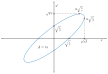
\includegraphics[width=0.8\linewidth,trim={0mm 0mm 0mm 0mm},clip]{figures/Twiss}
    \caption{\label{Fig:Twiss} The phase space ellipse of bunch particles. The figure is recreated from Figure 3.23 by Klauss Wille in \textit{The Physics of Particle Accelerators}~\cite{wille:2001}.}
\end{figure}

% ================================================================================================================================ %
\subsection{Extracting Twiss Parameters from Simulation Data}
\label{Apx:SA:EnTwiss:Sim}

Both OSIRIS and QuickPIC dump the macro particles as large arrays of six-dimensional data, providing each particle's position and momentum vector.
To study the collective motion of particles, it is useful to calculate the bunch total emittance in terms of the RMS value or standard deviation of its particles.
Equation~\ref{EQ:EmittFull} can be rewritten in terms of the statistical distributions of its particles such that
\begin{equation}
    \epsilon = \sqrt{\gamma\sigma_{x}^{2} + 2\alpha\sigma_{x}\sigma_{x^{\prime}} + \beta\sigma_{x^{\prime}}^{2}}, \label{EQ:Emitt}
\end{equation}
where the angle of the $i$-th particles can be taken from its momentum
\begin{equation}
    x_{i}^{\prime} = \frac{p_{i,x}}{p_{i,z}}.
\end{equation}

For a set of macro particles, the emittance can be calculated directly by taking the covariance matrix of the $x$ and $x^{\prime}$ vectors
\begin{equation}
    \mathbf{T} = \mathrm{cov}\left(\mathbf{x}, \mathbf{x}^{\prime}\right), \label{EQ:ECalc1}
\end{equation}
and then taking the square root of its determinant
\begin{equation}
    \epsilon = \sqrt{\mathrm{det}\left(\mathbf{T}\right)}. \label{EQ:ECalc2}
\end{equation}
The Twiss parameters can be extracted from the matrix $\mathbf{T}$ as well:
\begin{equation}
    \alpha = \mathrm{T}_{12}/\epsilon, \quad
    \beta  = \mathrm{T}_{11}/\epsilon, \quad
    \gamma = \mathrm{T}_{22}/\epsilon
\end{equation}

% ================================================================================================================================ %
\section{A Measure for Beam Quality}
\label{Apx:SA:QTilde}

For the emittance study in Publication~\ref{Pub:BL17}, it was necessary to define a convenient unit for the quality of the accelerated bunch in terms of emittance evolution in regions along the bunch length.
In the quasi-linear plus non-linear regime this publication investigates, emittance growth only occurs at the head of the bunch.
However, the region of emittance growth varies when parameters such as charge and beam size changes.
In the study, we defines the quantity
\begin{equation}
    \tilde{Q} = \sum_{m=0}^{M} \frac{1}{N} \left[\sum_{n=0}^{N} Q_{m+n}\right] \cdot \chi(\xi_{m},N),
\end{equation}
where $M$ is the number of longitudinal grid slices of length $\Delta\xi$ which contains macro particles for the witness bunch, and with corresponding coordinate $\xi_{m}$; $N$ is the number of such slices to average over; and $\chi(\xi_{m},N)$ is the step function
\begin{equation}
    \chi(\zeta,N) =
    \begin{cases}
        0, & \frac{\epsilon(\zeta) - \epsilon_{0}}{\epsilon_{0}} > 5\% \\
        1, & \frac{\epsilon(\zeta) - \epsilon_{0}}{\epsilon_{0}} \leq 5\%
    \end{cases}
    \quad\mathrm{for}\quad
    \xi_{m} < \zeta \leq \xi_{m} + N\Delta\xi,
\end{equation}
where $\epsilon(\zeta)$ is the emittance as defined by Equations~\ref{EQ:ECalc1} and~\ref{EQ:ECalc2} for a set of macro particles within the interval $\xi_{m}$ to $\xi_{m} + N\Delta\xi$.
For the studies included in Publication~\ref{Pub:BL17},
\begin{equation}
    M = \left\lfloor \frac{10\sigma_{z}}{\Delta\xi} \right\rceil, \quad
    N = 4.
\end{equation}
The first slice
\begin{equation}
    \xi_{0} = \mu_{\mathrm{eb}} - 5\sigma_{z,\mathrm{eb}} - 0.5\Delta\xi,
\end{equation}
where $\mu_{\mathrm{eb}}$ is the longitudinal centre of the bunch.

\paragraph{Note:} This method may yield a misleading result if the Twiss parameter $\alpha$ varies too much along the length of the bunch.
That is, the emittance can be locally small, and qualify for the $5\%$ criterion, even if the total emittance of the region included in $\tilde{Q}$ is not.
This can easily be checked after the seemingly optimal region of the bunch is known by verifying that its total emittance does not exceed the same criterion.

% ================================================================================================================================ %


% Publications

\part*{Publications}
\renewcommand\appendixtocname{Publications}
\renewcommand\appendixname{Publication}
\pagestyle{plain}

\appendix
    \renewcommand{\thechapter}{\Roman{chapter}}
    %
%  Publication 1 :: IPAC 2015
% ============================
%

\chapter{Loading of a Plasma-Wakefield Accelerator Section\\Driven by a Self-Modulated Proton Bunch}
\label{Pub:IPAC15}

\begin{hangparas}{10mm}{1}

    \textbf{Abstract:}
    Abstract

    \vspace{8mm}

    \textbf{Authors:}
    V. K. Berglyd Olsen, E. Adli (University of Oslo, Oslo, Norway)
    P. Muggli (Max Planck Institute for Physics, Munich, Germany and CERN, Geneva, Switzerland)
    J. M. Vieira (Instituto Superior Technico, Lisbon, Portugal)


    \vspace{5mm}

    \textbf{Publication:}
    Proceedings of IPAC 2015, Richmond, Virginia, USA

    \vspace{5mm}

    \textbf{Date:}

\end{hangparas}

    \includepdf[
        pages=1-last,
        openright,
        scale=0.95,
        pagecommand={}
    ]{files/IPAC15-WEPWA026.pdf}
    %
%  Publication 2 :: NAPAC 2016
% =============================
%

\chapter[Loading of Wakefields in a Plasma Accelerator Section Driven by a Self-Modulated\\Proton Beam,%
        ~\textit{Proceedings of NAPAC 2016}]%
        {\Large Loading of Wakefields in a Plasma Accelerator Section\\Driven by a Self-Modulated Proton Beam}
\label{Pub:NAPAC16}

\begin{description}

    \item[Abstract:]
    Using parameters from the AWAKE project and particle-in-cell simulations we investigate beam loading of a plasma
    wake driven by a self-modulated proton beam. Addressing the case of injection of an electron witness bunch after
    the drive beam has already experienced self-modulation in a previous plasma, we optimise witness bunch parameters of
    size, charge and injection phase to maximise energy gain and minimise relative energy spread and emittance of the
    accelerated bunch.

    \item[Authors:]
    Veronica K. Berglyd Olsen, Erik Adli (University of Oslo, Oslo, Norway),
    Patric Muggli (Max Planck Institute for Physics, Munich, Germany and CERN, Geneva, Switzerland),
    Jorge M. Vieira (Instituto Superior Technico, Lisbon, Portugal)

    \item[Publication:]
    Proceedings of NAPAC 2016, Chicago, Illinois, USA \cite{berglyd_olsen:2016}

    \item[Date:]
    9\ts{th} to 14\ts{th} of October, 2016

\end{description}

    \includepdf[
        pages=1-last,
        openright,
        scale=0.95,
        pagecommand={}
    ]{files/NAPAC16-TUA4CO03.pdf}
    %
%  Publication 4 :: IPAC 2017
% ============================
%

\chapter{Data Acquisition and Controls Integration of the AWAKE Experiment at CERN}
\label{Pub:IPAC17}

\begin{hangparas}{10mm}{1}

    \textbf{Abstract:}
    The AWAKE experiment has been successfully installed in the CNGS facility at CERN, and is
    currently in its first stage of operation. The experiment seeks to demonstrate self-modulation
    of an SPS proton beam in a rubidium plasma, driving a wakefield of several gigavolt per meter.
    We describe the data acquisition and controls system of the AWAKE experiment, its integration
    into the CERN controls system and new control developments specifically required for the AWAKE
    experiment.

    \vspace{8mm}

    \textbf{Authors:}
    Veronica K. Berglyd Olsen (University of Oslo, Oslo),
    Edda Gschwendtner (CERN, Geneva),
    Spencer Jake Gessner (SLAC, Menlo Park, California)

    \vspace{5mm}

    \textbf{Publication:}
    Proceedings of IPAC 2017, Copenhagen, Denmark

    \vspace{5mm}

    \textbf{Date:}

\end{hangparas}

    \includepdf[
        pages=1-last,
        openright,
        scale=0.95,
        pagecommand={}
    ]{files/IPAC17-TUPIK061.pdf}
    %
%  Publication 3 :: Peer Review
% ==============================
%

\chapter{Placeholder Title}
\label{Pub:PRev17}

\begin{hangparas}{10mm}{1}

    \textbf{Abstract:}
    Abstract

    \vspace{8mm}

    \textbf{Authors:}
    Veronica K. Berglyd Olsen (University of Oslo, Oslo)

    \vspace{5mm}

    \textbf{Publication:}
    Journal

    \vspace{5mm}

    \textbf{Date:}

\end{hangparas}


% Back Matters

\backmatter
\bibliography{Bibliography}
%~ \printbibliography
\null

\end{document}

% ==================================================================================================================== %
